\documentclass[11pt,a4paper]{article}

\usepackage[T1]{fontenc}
\usepackage[utf8]{inputenc}
\usepackage{lmodern}
\usepackage[margin=2.3cm]{geometry}
\usepackage{amsmath,amssymb}
\usepackage{graphicx}
\usepackage{booktabs}
\usepackage{tabularx}
\usepackage[font=small,labelfont=bf]{caption}
\usepackage[authoryear,round]{natbib}
\usepackage{microtype}
\usepackage{xcolor}
\usepackage[colorlinks=true,linkcolor=black,citecolor=blue!50!black,urlcolor=blue!50!black]{hyperref}

\graphicspath{{figures/}}
\newcommand{\pp}{\,pp}

\title{Sector-wise wake losses of the Kelmarsh wind farm from a lattice Boltzmann large-eddy simulation on a laptop GPU}
\author{Konrad Waleszczy\'nski\\[2pt]
  \small Independent researcher, Poland}
\date{Preprint, \today}

\begin{document}
\maketitle

\begin{abstract}
Wake losses of wind farms are usually estimated with engineering wake models, while large-eddy simulation (LES)
is considered too expensive for routine sector-by-sector comparisons with operational data. This paper presents a
compact lattice Boltzmann LES, written from published methods as a single module of GPU kernels in NVIDIA Warp,
and applies it to the six-turbine Kelmarsh onshore wind farm (United Kingdom) on a laptop GPU with 6\,GiB of
memory. The turbines are actuator disks in a neutral atmospheric boundary layer fed by a concurrent periodic
precursor. Seventy-two wind directions are simulated for each of two independent inflow realisations, and the
resulting power table is evaluated on exactly the same 159\,289 filtered ten-minute SCADA records (2016--2021) as
three engineering models in PyWake. The farm wake loss is 9.81\,\% in the LES (two standard errors 0.11\,\%),
9.24\,\% measured (95\,\% interval 8.98--9.52\,\%) and 9.69\,\% with the Gaussian model of Niayifar and
Port\'e-Agel. Over twelve 30-degree sectors the LES has the lowest root-mean-square error against the
measurements, 2.2 percentage points against 2.6 for the Gaussian, 3.7 for the Jensen and 4.4 for the TurbOPark
model, and the two inflow realisations agree within 0.52 points in every sector. All models overpredict the
losses of the four easterly sectors, the LES by 2.9--4.5 points. A per-turbine decomposition traces this to a
direction-dependent site effect on the free-stream reference turbine rather than to the wakes. One wind direction
takes 81\,s on the laptop GPU, a full sweep 1.7 GPU-hours. Code and result tables are openly available.
\end{abstract}

\section{Introduction}

Wake losses are one of the largest loss items in the energy yield of a wind farm, and they are almost always
estimated with engineering wake models: the top-hat model of \citet{jensen1983note} and \citet{katic1986cluster},
Gaussian models \citep{bastankhah2014gaussian,niayifar2016analytical} or models designed for clusters of farms
such as TurbOPark \citep{nygaard2020cluster,pedersen2022turbopark}. They run in milliseconds, but their wake
expansion and superposition rules carry empirical parameters, and different models applied to the same farm can
differ by several percentage points of annual loss. Comparisons with operational data are therefore usually made
per wind-direction sector, on measured power ratios of turbines in and out of wakes \citep{barthelmie2009offshore}.

Large-eddy simulation with actuator-disk or actuator-line rotors resolves the wakes and their interaction with
atmospheric turbulence from physical inputs alone \citep{calaf2010les,stevens2017review,porteagel2020review}. The
price is computational: a direction sweep of a real farm with turbulent inflow is usually a cluster job. The
lattice Boltzmann method (LBM) is local and memory-bound, which suits graphics processors well, and LBM-based LES
of wind-turbine wakes and of atmospheric boundary layers has been developed and assessed against established
Navier--Stokes solvers \citep{asmuth2020actuator,asmuth2021wall}.

This paper asks a practical question: can a consumer laptop GPU run an LES sweep of all wind directions of a real
farm, evaluated in exactly the same way as engineering models against SCADA data, with an honest estimate of its
own uncertainty? The test case is the Kelmarsh wind farm, whose SCADA data are openly published
\citep{plumley2025kelmarsh}. The contributions are:
\begin{itemize}
  \item a compact D3Q19 lattice Boltzmann LES with regularized collision, Smagorinsky closure, log-law wall model,
        filtered actuator disks and a concurrent precursor, verified against analytical solutions and momentum
        theory, in single and half precision;
  \item a direction sweep in which every turbine is referred to its own undisturbed inflow from a run without
        turbines, and whose power table goes through the same record selection, normalisation and sector
        aggregation as three PyWake models \citep{pedersen2019pywake};
  \item an uncertainty estimate from two independent inflow realisations, checked against the scatter of
        ten-minute blocks within each realisation;
  \item a per-turbine decomposition of the sector losses, which locates the largest common discrepancy of all
        models in the free-stream reference rather than in the wakes;
  \item the cost on a 6\,GiB laptop GPU, and openly available code and result tables.
\end{itemize}

\section{Site and SCADA data}
\label{sec:data}

Kelmarsh consists of six Senvion MM92 turbines (rotor diameter $D = 92$\,m, rated power 2.05\,MW) in
gently rolling farmland in Northamptonshire; turbines T3 and T6 have a hub height of 68.5\,m, the other four
78.5\,m. The dataset of \citet{plumley2025kelmarsh} provides ten-minute SCADA records and the turbine positions
under a CC-BY-4.0 licence. Ground elevation varies by about 20\,m across the farm; no terrain model is used in
this study.

The record selection and normalisation are those of an earlier engineering-model study of the same farm
\citep{waleszczynski2026wakeshadow}, imported unchanged (pinned version) rather than re-implemented. Records from
2016 to 2021 are kept when all six turbines run in partial load (power above 20\,kW, pitch below 5\textdegree) and
report a nacelle direction; the wind direction is the circular mean of the six. For each 1-degree direction the
free-stream turbines follow from the disturbed-sector rule of IEC~61400-12-1 \citep{iec61400121}. Each turbine
carries a site factor $c_i$, its power relative to the other free-stream turbines over the records in which it is
itself free, iterated to a fixed point with mean one; it removes the effect of hub height and position that holds
in all directions. With $\hat P_i = P_i / c_i$, the reference power of a record is the mean of $\hat P_i$ over its
free-stream turbines, and the reference wind speed follows from the inverse catalogue power curve. Records with a
reference speed between 5 and 10\,m/s are kept: 159\,289 records on 1\,913 days. The wake loss of a sector is
\begin{equation}
  L = 1 - \frac{\sum_{\mathrm{records}} \sum_{i=1}^{6} \hat P_i}{\sum_{\mathrm{records}} 6\, P_{\mathrm{ref}}} ,
  \label{eq:loss}
\end{equation}
over 30-degree sectors centred on 0, 30, \ldots, 330\textdegree. Its 95\,\% interval comes from a bootstrap of
whole days (1000 resamples), because ten-minute records within a day are strongly correlated. The ambient
turbulence intensity, the median ten-minute standard deviation of the nacelle anemometers over the mean speed,
is 12.7\,\%.

The models are evaluated on the same records: each record is looked up in a power table
$P_i(\mathrm{wd}, \mathrm{ws})$ at its own direction and reference speed, the model powers are normalised in the
same way, and Eq.~\eqref{eq:loss} is applied. The three PyWake models are the Jensen model with wake expansion
$k = 0.075$, the Gaussian model of \citet{niayifar2016analytical} and TurbOPark in the formulation of
\citet{pedersen2022turbopark}, all with the measured ambient turbulence intensity, the catalogue power curve of the
MM92 \citep{haas2024windpowerlib} and a generic thrust curve.

\section{Numerical method}
\label{sec:method}

\subsection{Lattice Boltzmann solver}

The solver uses the D3Q19 velocity set \citep{kruger2017lbm}, with one fused kernel per time step (pull
streaming, moments, forcing and collision) on two population arrays, written in NVIDIA Warp \citep{macklin2022warp};
the same kernels compile for the CPU, which is how the automated tests run. The collision is regularized BGK
\citep{latt2006regularized}: the non-equilibrium part of the populations is projected on the second-order Hermite
polynomials before relaxation, which keeps the scheme stable at the effectively infinite Reynolds number of the
atmosphere,
\begin{equation}
  f_q^{*} = f_q^{\mathrm{eq}} + \left(1 - \frac{1}{\tau}\right) f_q^{(1)} + \left(1 - \frac{1}{2\tau}\right) S_q ,
\end{equation}
with the forcing term $S_q$ of \citet{guo2002forcing} for all body forces (driving pressure gradient, wall stress
and rotor thrust). The first-order non-equilibrium moment $-\mathbf{F}/2$ has to be kept in $f^{(1)}$: a plain
second-order projection drops it and then delivers only $(3-\omega)/2$ of the force, which the Poiseuille test
below detected as 88\,\% of the expected flow rate at $\tau = 0.8$. The Smagorinsky eddy viscosity
\citep{smagorinsky1963} enters the relaxation time and is computed locally from the non-equilibrium momentum flux
$\Pi$ \citep{hou1994subgrid},
\begin{equation}
  \tau = \frac{1}{2}\left(\tau_0 + \sqrt{\tau_0^2 + 18\sqrt{2}\,(C_s \Delta)^2 \lVert \Pi \rVert / \rho}\right),
  \qquad C_s = 0.16 ,
\end{equation}
with the damping of \citet{mason1992backscatter} near the ground. Populations are stored as deviations from the
lattice weights, $f_q - w_q$, which keeps significant digits for the small deviations that carry the flow
\citep{lehmann2022precision}, in float32 or optionally float16.

\subsection{Atmospheric boundary layer and inflow}

The neutral surface layer is a pressure-driven open channel: a constant body force, a free-slip lid at 460\,m and
a rough ground represented by a log-law wall stress applied as a force in the first cell
\citep[local-velocity form, after][]{moeng1984les},
\begin{equation}
  \boldsymbol{\tau}_w = -\left[\frac{\kappa}{\ln(z_1/z_0)}\right]^2 \lvert \mathbf{U}_1 \rvert\, \mathbf{U}_1 ,
  \qquad z_1 = \Delta/2 , \quad \kappa = 0.4 .
\end{equation}
The roughness length $z_0 = 0.2$\,m (farmland with hedgerows and woods) was chosen so that the hub-height
turbulence intensity of the LES is close to the SCADA ambient value; it is the only parameter of the inflow that
was adjusted to the site. Coriolis forces, veer and thermal stratification are not modelled.

The inflow turbulence comes from a periodic precursor, 12\,$D$ long and as wide as the farm domain, whose wrap in
the streamwise direction is shifted laterally so that streaks do not lock in place \citep{munters2016shifted}.
It runs concurrently with the farm domain and hands over its outflow plane at every time step
\citep{stevens2014concurrent}; the farm domain has a zero-gradient outflow behind a 2\,$D$ sponge layer. The
precursor is spun up for 6000\,s of physical time before any farm run.

The farm domain is the same for every wind direction: the turbines are rotated into a wind-aligned frame around
the farm centre, with at least 5\,$D$ between the inflow plane and the nearest possible rotor, 5\,$D$ at the sides
and 10\,$D$ behind. Table~\ref{tab:setup} lists the main parameters. The LES is effectively Reynolds-number
independent and the disks use a constant thrust coefficient, so a run at one hub-height speed represents all
partial-load speeds; the lattice speed is mapped to 8\,m/s.

\begin{table}[htbp]
\centering
\caption{Simulation set-up of the main runs.}
\label{tab:setup}
\small
\begin{tabular}{ll}
\toprule
Grid spacing & $\Delta = D/8 = 11.5$\,m (D/12 and D/16 in the grid study) \\
Farm domain & $213 \times 173 \times 40$ cells ($2.45 \times 1.99 \times 0.46$\,km) \\
Precursor & $96 \times 173 \times 40$ cells (12\,$D$ long), shifted periodic \\
Cells in total & 2.14 million \\
Hub-height speed & 0.05 in lattice units (Mach number 0.09), mapped to 8\,m/s \\
Time step & 0.069\,s; about 35\,000 steps per direction \\
Run & 10\,min spin-up, 30\,min average in three 10-minute blocks \\
Directions & 72 (every 5\textdegree), two inflow realisations \\
Disks & $C_T = 0.8$, $C_T' = 1.388$ (calibrated), Gaussian width $\sigma = 0.75\Delta$ \\
Subgrid model & Smagorinsky, $C_s = 0.16$, Mason--Thomson wall damping \\
Ground & log-law wall model, $z_0 = 0.2$\,m; free-slip lid at 460\,m \\
\bottomrule
\end{tabular}
\end{table}

\subsection{Actuator disks}

The rotors are thrust-only disks normal to the mean wind, smoothed with a Gaussian of width $\sigma = 0.75$ cells
along the axis and an error-function edge in the rotor plane. The thrust uses the disk-averaged velocity
$\langle u_d \rangle$ of the previous step and the local thrust coefficient $C_T'$ \citep{calaf2010les}, with the
correction for filtered disks of \citet{shapiro2019filtered},
\begin{equation}
  F = -\tfrac{1}{2}\rho\, C_T' M^2 \langle u_d \rangle^2 A ,
  \qquad M = \left(1 + \frac{C_T'\,\Delta_f}{4\sqrt{3\pi}\,R}\right)^{-1},
  \qquad \Delta_f = \sqrt{12}\,\sigma .
\end{equation}
$C_T'$ is calibrated per resolution so that an isolated disk in uniform inflow gives $C_T = 0.8$, the
partial-load thrust coefficient of the generic thrust curve (no thrust curve of the MM92 is public). The
calibration gives $C_T' = 1.388$ at $D/8$ and 1.427 at $D/12$, against 1.528 from momentum theory, and the
ratio $r = \langle u_d \rangle / U_\infty = 0.814$ at $D/8$, which turns a disk velocity into a free-stream
equivalent speed $\langle u_d \rangle / r$ for the power curve.

\subsection{Runs and the reference without turbines}

Each direction is a 10-minute spin-up followed by a 30-minute average, split into three SCADA-like ten-minute
blocks. All directions of one inflow realisation start from the same spun-up precursor state and the solver is
deterministic, so they see the same inflow turbulence (common random numbers), which suppresses most
direction-to-direction sampling noise.

A 30-minute mean of the inflow is not uniform. Long-lived streaks leave the mean hub-height speed varying from
0.89 to 1.07 of the inflow hub speed across the domain (standard deviation 3.6\,\%; 0.90--1.03 and 2.3\,\% in the
second realisation). Referring every turbine to the farm-wide inflow speed turned this into $\pm 15$\,\% of power
and negative wake losses in some sectors. Because the inflow is identical in every run of a realisation, one
extra run without turbines gives the undisturbed mean velocity at every possible rotor position. The equivalent
speed ratio of turbine $i$ in block $b$ is therefore
\begin{equation}
  s_{i,b} = \frac{\langle u_{d,i} \rangle_b}{r\, \langle u_{d,i}^{\,0} \rangle_b}\, h_i ,
\end{equation}
where $u^{0}$ is the same disk average in the run without turbines and $h_i$ the shear factor of hub height
$i$ (68.5 or 78.5\,m) relative to the reference height. With this reference the free-stream turbines run at
$0.997 \pm 0.013$ of their own undisturbed inflow over 219 turbine-directions ($0.998 \pm 0.013$ in the second
realisation).

\subsection{From speed ratios to wake losses}

Because the flow scales with the wind speed, the LES gives the power table
\begin{equation}
  P_i(\mathrm{wd}, \mathrm{ws}) = \frac{1}{N_b}\sum_{b} P_{\mathrm{curve}}(\mathrm{ws}\, s_{i,b}) ,
\end{equation}
averaged over the $N_b = 6$ blocks of both realisations and interpolated linearly between the 5-degree
directions. It enters the evaluation of Sect.~\ref{sec:data} in place of a PyWake table. Sampling directions every
5 instead of 1 degree changes the sector losses of the Gaussian model by at most 0.18 points and its farm loss by
less than 0.01 points.

The uncertainty of the LES loss is the standard error over blocks: the loss of Eq.~\eqref{eq:loss} is evaluated
with each block alone, and the standard deviation of the six results is divided by $\sqrt 6$. This treats the
three blocks of one realisation as independent, which the second realisation tests (Sect.~\ref{sec:realisations}).

\section{Verification}
\label{sec:verification}

Table~\ref{tab:verification} and Fig.~\ref{fig:verification} summarise the checks. The viscosity recovered from
the decay of a Taylor--Green vortex converges at second order, the body-force-driven Poiseuille flow is reproduced
to about 1\,\%, and an actuator disk in uniform inflow follows momentum theory closely at both resolutions; at a
local thrust coefficient of 1.5 the induction is 0.255 at $D/8$ and 0.262 at $D/16$ against 0.273 from theory.
The precursor reproduces the log law in the first cell (mean speed 8.45 against 8.40 $u_*$), while the hub-height
speed lies 4\,\% below it, the log-layer mismatch typical of wall-modelled LES with a Smagorinsky closure
\citep{brasseur2010loglayer}. The resolved shear stress reaches 0.93\,$u_*^2$ at 40\,m, and the hub-height
turbulence intensity is 13.4\,\% (12.9\,\% in the second realisation) against 12.7\,\% from the SCADA.

\begin{table}[htbp]
\centering
\caption{Verification and sensitivity checks.}
\label{tab:verification}
\small
\begin{tabularx}{\textwidth}{>{\raggedright\arraybackslash}p{0.33\textwidth}X}
\toprule
Check & Result \\
\midrule
Taylor--Green vortex, viscosity from energy decay, 16/32/64/128 cells per wavelength & error 10.0 / 2.5 / 0.70 / 0.29\,\%, second order \\
Poiseuille channel (body force, bounce-back walls), 8/16/32 cells, $\tau = 0.8$ & maximum profile error 1.1 / 1.1 / 0.23\,\% \\
Actuator disk in uniform inflow, $C_T' = 1.5$, $D/8$ and $D/16$ & induction 0.255 / 0.262 (theory 0.273); $C_T$ 0.832 / 0.817 (theory 0.793) \\
Inflow profile, $D/8$ & first cell 8.45 $u_*$ (log law 8.40); hub 4\,\% below the log law; resolved shear stress 0.93 $u_*^2$ at 40\,m \\
Inflow turbulence at hub height & TI 13.4\,\% and 12.9\,\% (SCADA 12.7\,\%); $\sigma_u, \sigma_v, \sigma_w$ = 1.9, 1.4, 1.1 $u_*$ \\
Direction step of 5\textdegree\ instead of 1\textdegree\ (Gaussian model) & sector losses change by at most 0.18\pp, farm loss by less than 0.01\pp \\
Grid, 240\textdegree\ and 300\textdegree, $D/8$, $D/12$, $D/16$ & loss at 8\,m/s: 19.5 / 18.5 / 20.5\,\% and 30.5 / 28.8 / 29.6\,\%; hub TI 13.4 / 12.4 / 12.5\,\% \\
float16 populations & Taylor--Green error 0.76 / 0.60\,\% at 64 / 128 cells; farm loss at 240\textdegree\ 19.9 against 19.5\,\%, every speed ratio within 0.017 of float32 \\
\bottomrule
\end{tabularx}
\end{table}

\begin{figure}[htbp]
\centering
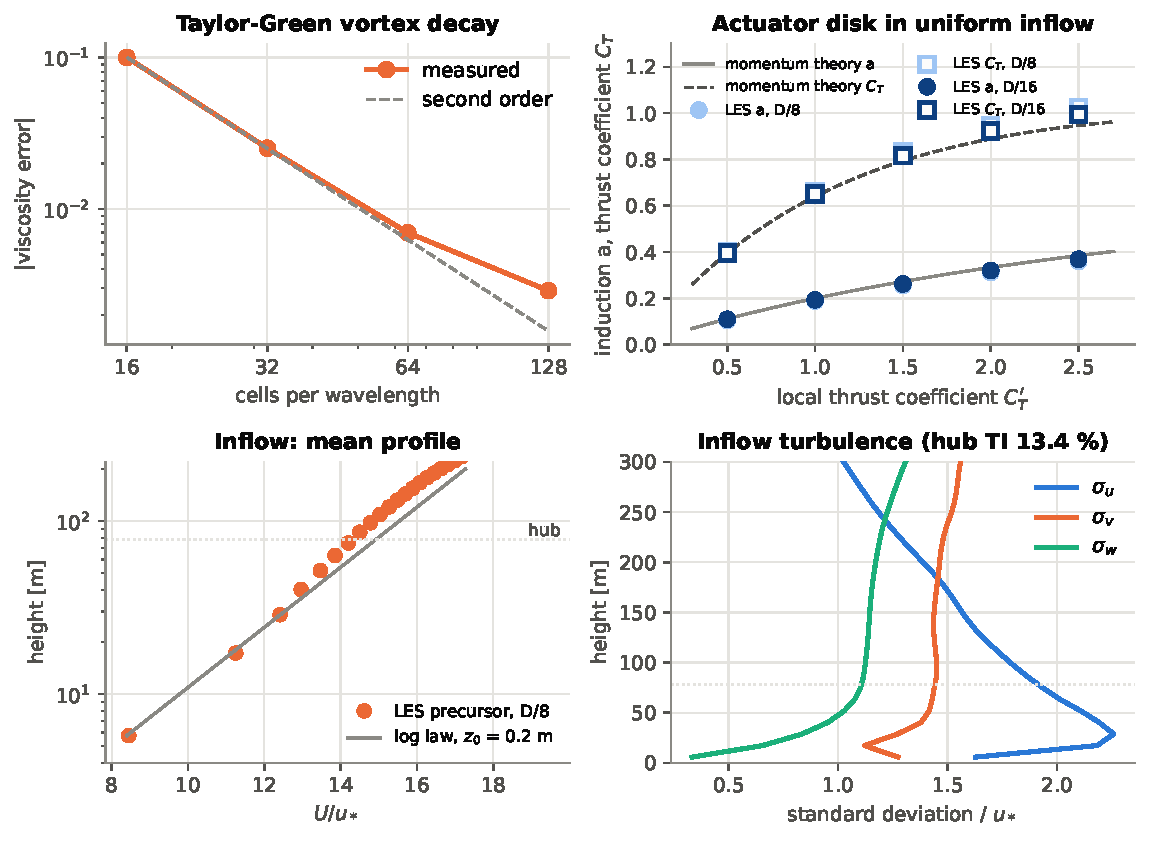
\includegraphics[width=0.84\textwidth]{verification.pdf}
\caption{Verification. Top left: viscosity error of the Taylor--Green vortex. Top right: induction and thrust
coefficient of an isolated actuator disk against momentum theory. Bottom: mean velocity and turbulence profiles of
the precursor at $D/8$ (dotted line: hub height).}
\label{fig:verification}
\end{figure}

\paragraph{Grid study.} The two directions with the deepest wakes, 240\textdegree\ and 300\textdegree, were
repeated at 12 and 16 cells per rotor diameter, each resolution with its own disk calibration and precursor. The
farm loss of one direction at 8\,m/s (farm power over six times the mean power of the free-stream turbines) is
19.5, 18.5 and 20.5\,\% at 240\textdegree\ and 30.5, 28.8 and 29.6\,\% at 300\textdegree\ for $D/8$, $D/12$ and
$D/16$. The changes are within one to two standard errors of the ten-minute blocks (0.2--1.2 points) and show no
trend. Because every resolution has its own turbulence realisation, the study cannot resolve differences below
about one point.

\paragraph{Half precision.} With float16 populations the Taylor--Green errors stay below 1\,\% and the farm loss
at 240\textdegree\ changes from 19.5 to 19.9\,\%, each turbine's speed ratio within 0.017 of its float32 value.
Half precision halves the memory and raises the kernel throughput by about 6\,\% (Sect.~\ref{sec:cost}); all
results below use float32.

\section{Results}
\label{sec:results}

\subsection{Flow field}

Figure~\ref{fig:hub} shows the hub-height flow for the two directions with the deepest wakes. At 300\textdegree\
the turbines stand in two rows, T3--T5--T6 and T2--T1--T4, whose wakes merge downstream; at 240\textdegree\ three
pairs stand one behind the other (T2--T3, T1--T5, T4--T6). The instantaneous fields show the wakes meandering in
the streaky inflow.

\begin{figure}[htbp]
\centering
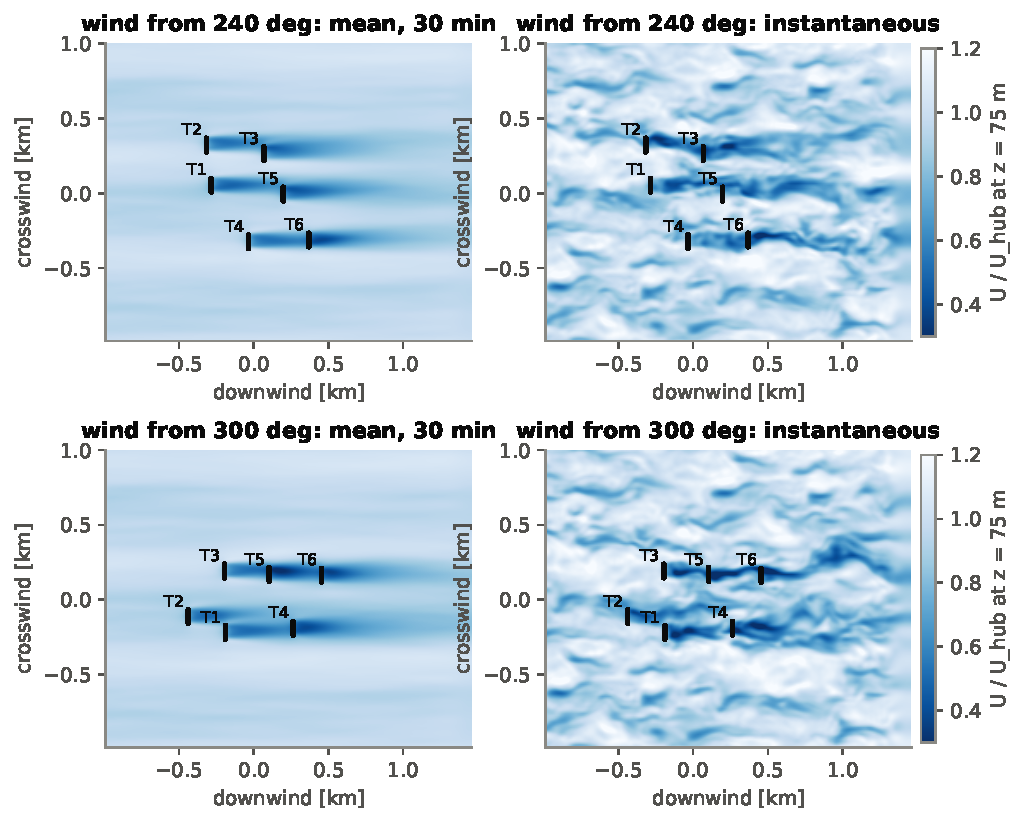
\includegraphics[width=0.84\textwidth]{hub_plane.pdf}
\caption{Streamwise velocity at $z = 75$\,m, the grid level nearest to the 78.5\,m hub height, for wind from
240\textdegree\ (top) and 300\textdegree\ (bottom): 30-minute mean (left) and an instantaneous field (right),
normalised by the inflow hub speed.}
\label{fig:hub}
\end{figure}

\subsection{Wake loss per sector}

Table~\ref{tab:sectors} and Fig.~\ref{fig:sectors} compare the wake losses. The LES farm loss, 9.81\,\%, lies
0.6 points above the measured 9.24\,\% and close to the Gaussian model (9.69\,\%), while Jensen and TurbOPark
overpredict by 2.2 and 2.9 points. Over the twelve sectors the LES has the lowest root-mean-square error and the
smallest mean bias. The deep-wake sectors are reproduced: along the row T3--T5--T6 at 300\textdegree\ the LES
gives 22.1\,\% against 22.2\,\% measured, where the Gaussian model is 1.9 points low and Jensen and TurbOPark 1.3
and 2.8 points high. At 240\textdegree, the most frequent sector, the LES is 1.1 points low. Figure~\ref{fig:eff}
resolves the farm efficiency in 5-degree bins.

\begin{table}[htbp]
\centering
\caption{Wake loss per 30-degree sector [\%] on the same SCADA records. SCADA with its 95\,\% day-bootstrap
interval; LES pooled over two inflow realisations with two standard errors of its six ten-minute blocks, and
each realisation on its own (r0 / r1).}
\label{tab:sectors}
\small
\begin{tabular}{rrlllccc}
\toprule
Sector & Records & SCADA [95\,\%] & LES $\pm$ 2\,SE & r0 / r1 & Gaussian & Jensen & TurbOPark \\
\midrule
0\textdegree & 7\,120 & 5.4 [5.0--5.7] & 4.8 $\pm$ 0.3 & 4.8 / 4.7 & 5.2 & 6.0 & 6.4 \\
30\textdegree & 10\,791 & 3.3 [2.7--3.8] & 3.7 $\pm$ 0.3 & 3.6 / 3.9 & 4.9 & 6.0 & 5.8 \\
60\textdegree & 7\,733 & 7.8 [6.9--8.6] & 10.7 $\pm$ 0.3 & 10.8 / 10.6 & 11.0 & 13.3 & 14.5 \\
90\textdegree & 6\,041 & 2.1 [1.4--2.9] & 6.6 $\pm$ 0.3 & 6.6 / 6.7 & 7.4 & 8.6 & 9.8 \\
120\textdegree & 4\,622 & 19.7 [18.8--20.7] & 22.8 $\pm$ 0.5 & 22.7 / 22.9 & 20.9 & 24.4 & 25.4 \\
150\textdegree & 6\,606 & 5.9 [5.5--6.3] & 9.6 $\pm$ 0.3 & 9.7 / 9.4 & 10.3 & 11.7 & 12.3 \\
180\textdegree & 14\,731 & 3.7 [3.4--4.1] & 5.2 $\pm$ 0.4 & 4.9 / 5.4 & 5.7 & 6.6 & 7.1 \\
210\textdegree & 28\,137 & 3.9 [3.7--4.1] & 5.6 $\pm$ 0.2 & 5.7 / 5.5 & 5.4 & 6.5 & 6.5 \\
240\textdegree & 29\,728 & 14.4 [14.0--14.8] & 13.3 $\pm$ 0.7 & 13.3 / 13.3 & 12.4 & 14.9 & 16.1 \\
270\textdegree & 19\,019 & 8.2 [7.9--8.5] & 7.1 $\pm$ 0.4 & 7.1 / 7.1 & 7.4 & 8.9 & 9.5 \\
300\textdegree & 16\,219 & 22.2 [21.7--22.7] & 22.1 $\pm$ 0.6 & 22.1 / 22.1 & 20.3 & 23.5 & 25.0 \\
330\textdegree & 8\,542 & 9.0 [8.7--9.4] & 9.7 $\pm$ 0.4 & 9.6 / 9.8 & 10.9 & 12.2 & 12.7 \\
\midrule
all & 159\,289 & 9.24 [8.98--9.52] & 9.81 $\pm$ 0.11 & 9.79 / 9.83 & 9.69 & 11.44 & 12.13 \\
RMSE & & & 2.2 & 2.2 / 2.2 & 2.6 & 3.7 & 4.4 \\
bias & & & $+1.3$ & $+1.3$ / $+1.3$ & $+1.4$ & $+3.1$ & $+3.8$ \\
\bottomrule
\end{tabular}
\end{table}

\begin{figure}[htbp]
\centering
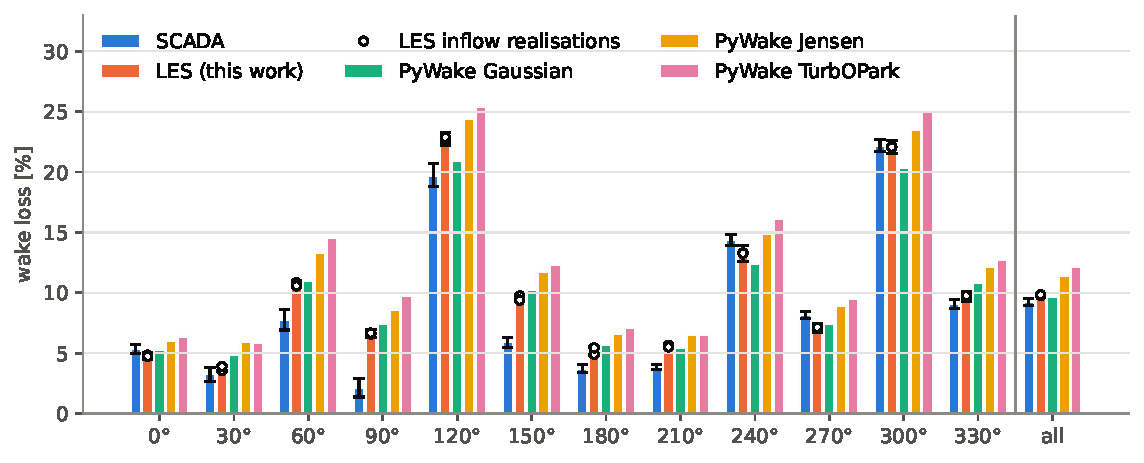
\includegraphics[width=\textwidth]{sector_losses.pdf}
\caption{Wake loss per sector. Whiskers: SCADA 95\,\% day-bootstrap interval; LES two standard errors of its six
ten-minute blocks from two inflow realisations. Circles: the two realisations on their own.}
\label{fig:sectors}
\end{figure}

\begin{figure}[htbp]
\centering
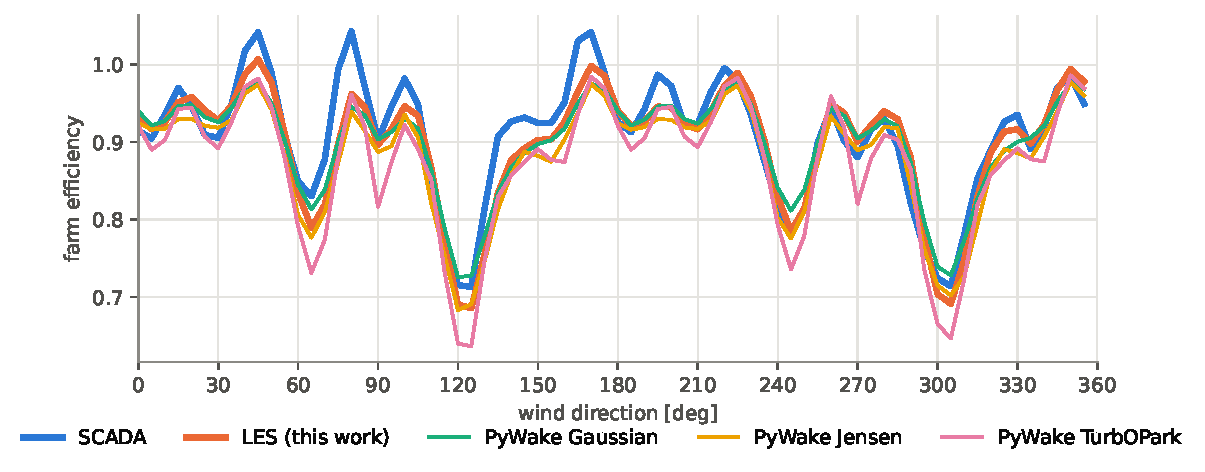
\includegraphics[width=0.9\textwidth]{efficiency_direction.pdf}
\caption{Farm efficiency (one minus the wake loss) in 5-degree bins with at least 100 records. The measured curve
rises above one in a few directions, a site effect that the site factors only partly remove; at 60--80\textdegree\
and 130--160\textdegree\ every model stays below the measurement.}
\label{fig:eff}
\end{figure}

\subsection{Inflow realisations and the uncertainty of the LES}
\label{sec:realisations}

The second realisation repeats the whole chain with a precursor started from a different random seed, its own run
without turbines and the same 72 directions. Its farm loss is 9.83\,\% against 9.79\,\% for the first, its
sector-wise RMSE and bias against the SCADA are the same, and no sector differs by more than 0.52 points (root
mean square over the sectors 0.24 points). If the ten-minute blocks of a realisation were less independent than
assumed, the two realisations would differ by more than their block scatter predicts; the block standard errors
predict a root-mean-square difference of 0.44 points, larger than observed. The block-based interval, 0.2--0.7
points per sector and 0.11 points on the farm loss, is therefore not optimistic. Two realisations are enough for
this check but not to estimate the between-realisation spread on its own.

\subsection{Turbine by turbine: the easterly sectors}
\label{sec:turbines}

Every model, the LES included, overpredicts the losses of the four easterly sectors (60--150\textdegree), the LES
by 2.9--4.5 points. Because the farm loss of a sector is the mean of the six turbine losses against the same
reference, Eq.~\eqref{eq:loss} splits exactly into turbines. Averaged over the four sectors, most of the LES excess
comes from T2 (11.3 points of turbine loss) and T1 (5.4 points); T3, T4 and T5 are within 2.4 points and T6
is 1.9 points below the measurement. The Gaussian model shows the same pattern (T2 9.6, T1 6.7, T6 $-3.5$
points).

Figure~\ref{fig:turbines} shows why. The wake minima agree: at 140\textdegree\ T2 produces 0.33 of the reference
power in the SCADA and 0.34 in the LES. What differs is the level outside the wakes. In the 5-degree bins where
neither the LES nor the Gaussian model sees a wake on a turbine (Table~\ref{tab:unwaked}), the measured turbines
T2 and T3 produce 6 and 5\,\% more than the free-stream reference in easterly winds and T6 6\,\% less, while in
westerly winds T1--T5 are within 1\,\% of it. T6 is one of the reference turbines in every easterly direction, so
the reference itself is low there and the measured losses come out small. A single site factor per turbine cannot
remove such an effect: T6 is 6\,\% low in easterly and 7\,\% high in westerly winds, and its factor averages the
two. A direction-dependent effect of this size is absent from flat-terrain models; terrain, roughness changes or
obstacles upwind of T6 are plausible causes that this study cannot separate.

\begin{figure}[htbp]
\centering
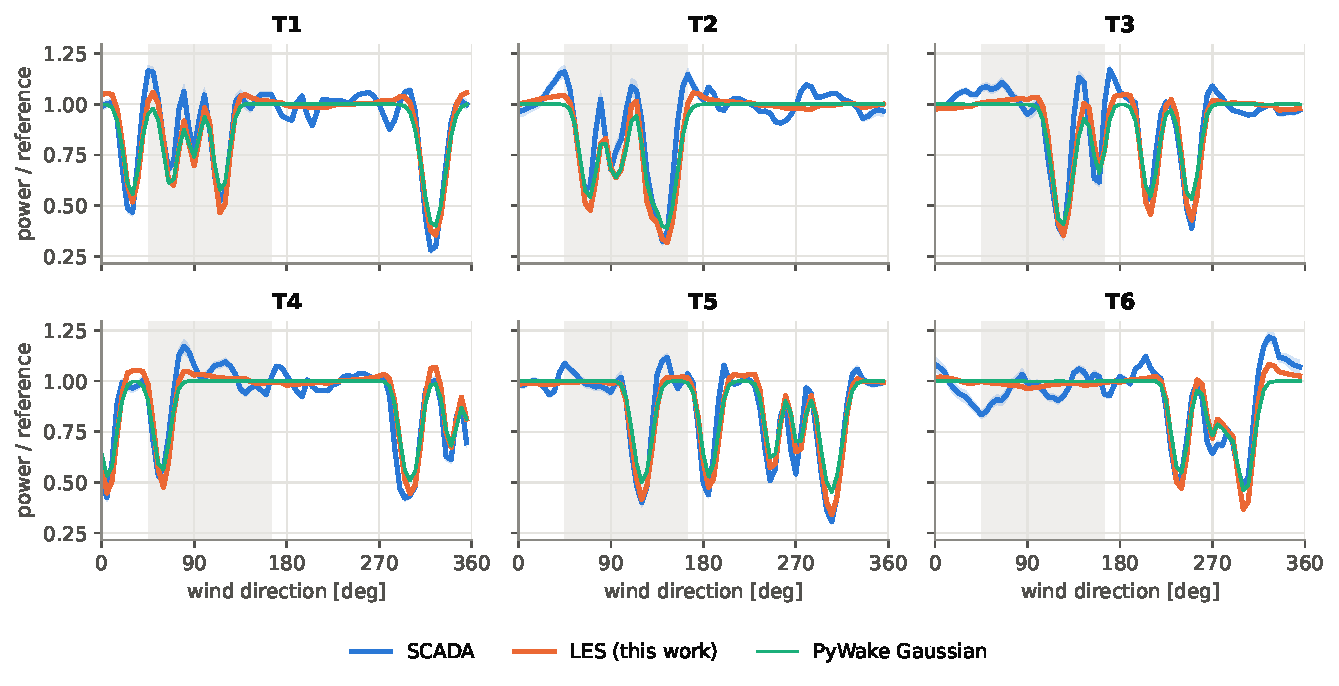
\includegraphics[width=0.94\textwidth]{turbine_efficiency.pdf}
\caption{Power of each turbine relative to the free-stream reference in 5-degree bins (SCADA with its 95\,\%
interval over days). Shaded: the easterly sectors 60--150\textdegree.}
\label{fig:turbines}
\end{figure}

\begin{table}[htbp]
\centering
\caption{Power of unwaked turbines relative to the free-stream reference: record-weighted mean over the 5-degree
bins with at least 300 records in which neither the LES nor the Gaussian model sees a wake on the turbine
(ratio above 0.99).}
\label{tab:unwaked}
\small
\begin{tabular}{lcccccc}
\toprule
 & T1 & T2 & T3 & T4 & T5 & T6 \\
\midrule
SCADA, easterly winds (0--175\textdegree) & 1.01 & 1.06 & 1.05 & 1.03 & 1.02 & 0.94 \\
SCADA, westerly winds (180--355\textdegree) & 1.01 & 1.00 & 1.00 & 1.00 & 1.00 & 1.07 \\
LES, easterly winds & 1.02 & 1.03 & 1.02 & 1.02 & 1.00 & 1.00 \\
LES, westerly winds & 1.01 & 1.00 & 1.01 & 1.00 & 1.02 & 1.02 \\
\bottomrule
\end{tabular}
\end{table}

\subsection{Single wake}

Behind a single turbine in the same inflow (Fig.~\ref{fig:wake}) the LES centreline deficit, relative to the same
position in the run without turbines, is deeper than in the Gaussian and Jensen models up to about 8\,$D$ (0.32
against 0.26 and 0.22 at 4\,$D$) and recovers to 0.11 at 10\,$D$. The TurbOPark centreline deficit in PyWake stays
much deeper (0.46 at 4\,$D$), consistent with its overprediction of the farm loss.

\begin{figure}[htbp]
\centering
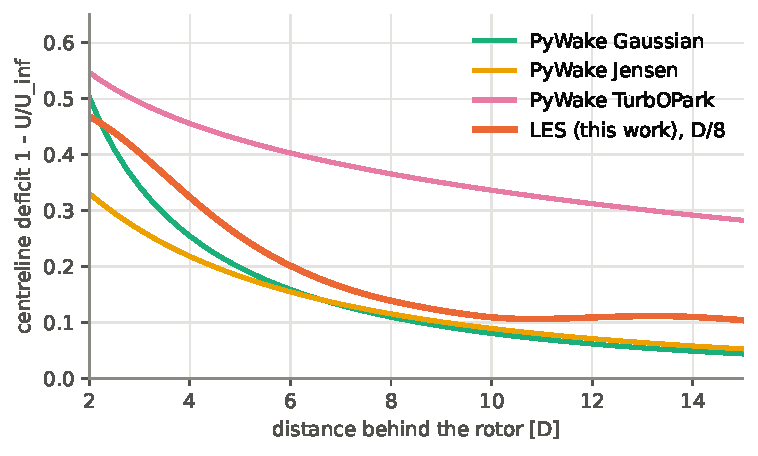
\includegraphics[width=0.55\textwidth]{wake_deficit.pdf}
\caption{Hub-height centreline velocity deficit behind a single turbine: LES at $D/8$ and the PyWake models at the
LES inflow turbulence intensity.}
\label{fig:wake}
\end{figure}

\subsection{Computational cost}
\label{sec:cost}

The laptop GPU is an NVIDIA Quadro RTX 3000 (Turing, 6\,GiB). The bare float32 kernel runs at 1240--1320 million
lattice updates per second (MLUPS) from 0.3 to 19 million cells (2.7\,GiB of populations); with float16 storage it
reaches 1340 MLUPS and fits 37 million cells in 2.6\,GiB (Fig.~\ref{fig:cost}). A farm run, farm domain and
precursor together with 2.14 million cells, runs at about 920 MLUPS including disk forces and averaging: 81\,s per
wind direction, 1.7 GPU-hours for 72 directions and below 1.5\,GiB of GPU memory. Each further realisation costs
the same again. At $D/12$ and $D/16$ one direction takes 413 and 1290\,s with 2.1 and 3.6\,GiB, so a full sweep at
$D/16$ would take about 26 GPU-hours.

\begin{figure}[htbp]
\centering
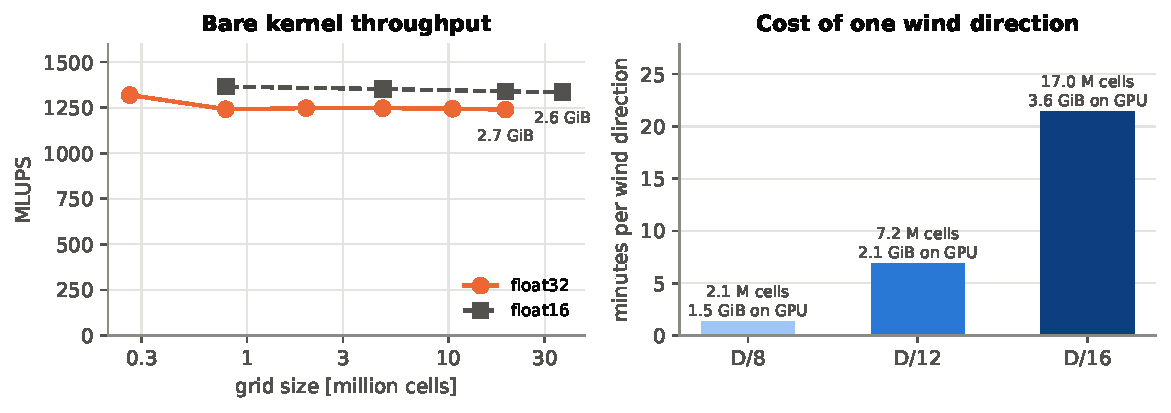
\includegraphics[width=0.86\textwidth]{performance.pdf}
\caption{Left: throughput of the bare kernel against grid size (labels: memory of the populations). Right: wall
time of one wind direction (10-minute spin-up and 30-minute average) at three resolutions.}
\label{fig:cost}
\end{figure}

\section{Limitations}
\label{sec:limitations}

\begin{itemize}
  \item \emph{Neutral, flat, no Coriolis.} No veer, stability or terrain. The easterly sectors show a
        direction-dependent site effect on the free-stream turbines that none of the models contains.
  \item \emph{Coarse rotors.} At $D/8$ the rotor spans eight cells and the hub lies seven cells above the ground.
        The disks are calibrated to the right thrust, and up to $D/16$ the loss changes by about one point without
        a trend, but the grid study covers two directions, cannot separate resolution from turbulence realisation
        below that level and does not resolve the near wake.
  \item \emph{One wind speed.} The LES runs with $C_T = 0.8$ and is scaled to the 5--10\,m/s records; the generic
        thrust curve falls to 0.71 at 10\,m/s, so the fastest records are slightly over-thrusted.
  \item \emph{Thrust-only disks, perfectly yawed.} No rotation, nacelle or tower, no yaw misalignment.
  \item \emph{Two inflow realisations.} Enough to test the block-based uncertainty, not to estimate the
        between-realisation spread with precision.
  \item \emph{Different averaging.} The LES turbulence intensity is a 30-minute standard deviation of the resolved
        field, the SCADA value the median ten-minute standard deviation of nacelle anemometers.
\end{itemize}

\section{Conclusions}

A lattice Boltzmann LES written from published methods runs a complete 72-direction sweep of a six-turbine onshore
farm in 1.7 hours on a 6\,GiB laptop GPU. Evaluated on exactly the same SCADA records and with the same
normalisation as three engineering wake models, it gives a farm wake loss of 9.81\,\% against 9.24\,\% measured and
the lowest sector-wise error of the four, without a wake parameter fitted to the losses. Its inputs are a
roughness length, a thrust coefficient and the turbine positions, and the first two are chosen rather than
measured: the roughness length so that the hub-height turbulence intensity is close to the SCADA ambient value,
and the disk coefficient $C_T'$, calibrated per resolution, so that an isolated disk reproduces the thrust
coefficient of a generic thrust curve. Neither is fitted to the measured wake losses. Two ingredients made the
comparison meaningful at this cost: referring every turbine to its own undisturbed inflow from a run without
turbines, which removes the bias of long-lived streaks, and a second inflow realisation, which showed that the
block-based uncertainty is not optimistic. The largest common error of all models, in the easterly sectors, is not
a wake error: the per-turbine decomposition places it in a direction-dependent site effect on the free-stream
reference turbine, which a single site factor per turbine cannot remove. For SCADA-based wake-loss assessments
this suggests checking the unwaked levels of the reference turbines direction by direction before attributing a
model discrepancy to the wake model.

\section*{Code and data availability}

The solver, the analysis and all result tables are available under the MIT licence at\\
\url{https://github.com/kwwaleszczynski-del/wind-les-gpu} \citep{waleszczynski2026windles}; the numbers in this
paper correspond to commit 3fe934a. The SCADA record selection and the PyWake models are
taken from \citet{waleszczynski2026wakeshadow} (commit 2bb9f11). The Kelmarsh data are available from Zenodo
\citep{plumley2025kelmarsh} under CC-BY-4.0.

\section*{Acknowledgements}

The author thanks Cubico Sustainable Investments for publishing the Kelmarsh wind farm data, DTU Wind Energy for
PyWake and NVIDIA for Warp.

\section*{Competing interests}

The author declares no competing interests.

\bibliographystyle{plainnat}
\bibliography{references}

\end{document}
